%TODO: fix citations.
%TODO: review results
%TODO: outline conclusions
%TODO: write introduction
%TODO: write methodology
%TODO: re-write results
%TODO: write conclusions
%TODO: review extensively
\documentclass[letterpaper]{sig-alternate}

\usepackage{hyperref}

\pdfpagewidth=8.5in
\pdfpageheight=11in

%\usepackage[factor=250,spacing=true]{microtype}

\begin{document}
\conferenceinfo{RecSys '14}{October 6--10, 2014, Foster City, Silicon Valley, USA}
%\CopyrightYear{2007} % Allows default copyright year (20XX) to be over-ridden - IF NEED BE.
%\crdata{0-12345-67-8/90/01}  % Allows default copyright data (0-89791-88-6/97/05) to be over-ridden - IF NEED BE.

\title{TODO: title}

\numberofauthors{2}

\author {
\alignauthor
Daniel Kluver\\
\affaddr{GroupLens Research}\\
\affaddr{Department of Computer Science and Engineering}\\
\affaddr{University of Minnesota}\\
\affaddr{Minneapolis, MN 55455 USA}\\
\email{kluver@cs.umn.edu}
\alignauthor
Joseph A. Konstan\\
\affaddr{GroupLens Research}\\
\affaddr{Department of Computer Science and Engineering}\\
\affaddr{University of Minnesota}\\
\affaddr{Minneapolis, MN 55455 USA}\\
\email{konstan@cs.umn.edu}
}

\maketitle
\begin{abstract}

TODO: abstract

\end{abstract}

%TODO: update these things.
% A category with the (minimum) three required fields
\category{H.4}{Information Systems Applications}{Miscellaneous}
%A category including the fourth, optional field follows...
\category{D.2.8}{Software Engineering}{Metrics}[complexity measures, performance measures]

%TODO: update these things.
\terms{Theory}

%TODO: update these things.
\keywords{ACM proceedings, \LaTeX, text tagging}

\section{Introduction}
  % describe new user experience in in recommender systems.
  One of the important problems in recommender systems is the new user experience.
  Most recommenders only have one chance to impress new users.
  If the user doesn't like the system, the user will leave.
  Even if the user stays, how the recommender system behaves for these new users can set the user's expectations for how the system will work in the future.
  

  % new user experience is important, and here is why.
    % talk about first impressions and user trust
    % How an algorithm behaves the first time a user sees it is important (first impression)
  The user's first impression of the system can be very important in teaching the user to trust the system.
  If the recommendation system does not perform well, the user will not trust its recommendations.
  User trust in recommenders is a complex issue.
  %TODO: re-skim the trust article.


%%%%%%%%%%%%%%%%%%%%%%
  This is especially a concern with recommender systems which rely on large amounts of user information to make personalization decisions.
  When users are new the system will not have much information to personalize the user experience which may lead the user to leave the system.
%%%%%%%%%%%%%%%%%%%%%%

  % past work tends to focus on the algorithm side, the algorithm side of this problem is cold start.
    % cold start algorithms is a larger problem
    % cold start algorithms tend to use extra information to help imrpove eary performance.
    % we only look at user cold start as it is ubiquitous.
  Past work on new user experiance in recommender systems has tended to focus on the algorithmic cold start problem.
  

  % One common new user strategy is to have a special data collection mode.
  % collect ratings fast to get over a precived ``bad period''
  % work on this focuses on how to collect useful ratings.
  % (framework from decision tree work)
  The best studied strategy for new users is to have users go through a new user rating survey.

  % One promising approach is to let user control interaction
  % user or system driven control.
  % promising, we don't know much about follow up.
  One promissing approach to new users is to have users control the new user rating survey.

  % bridge from past work to our work.
    % point out holes (evaluating standard algorithms for little to no ratings, wholeistic evaluation)
    % point out that other approaches than smart object ordering exist, and we need to be able to compare.
    % cite the comparison work at CHI.
  While past work has covered the new user rating survey as a solution to new user cold start, much less work has been done comparing other strategies.

  % Temporal evaluation
    % similar in-so-much as it can provide similar answers (growth over time), 
    % different in-so-much as it tends to be used for just system growth, but it could be used for user growth.
  Some researchers have taken to perfforming temporal evaluations of recommender systems, looking at accuracy metrics as a function of the lifetime of a system.
  
  %TODO: restructure this, I can't have my cake and eat  too. This needs ot be refocused to explicitly focus on similarities and differences.
  %One related approach to the one we take here is to evaluate recommender systems temporally.
  %Various authors have taken this approach \cite{KorenTemporal, LathiaTemporal, burke2010evaluating} to evaluating recommender systems to understand how recommenders change with time.
  %This work often features similar evaluations to ours, focusing on time (life of user or life of system) as opposed to number of ratings.
  %One major difference between this approach and the one we take is that using ratings in the order that they were given can expose algorithms to biases from the system they were collected in.
  %For example, in the MovieLens system users enter their first 15 ratings in a different interface, which does not give them choice over which items to rate.
  %This is a forced situation which produces qualitatively different ratings than normal ratings.
  %For this work we want to avoid this effect and therefor must use randomization.
  %TODO: SOMEWHERE AROUND HERE THIS GOES!


  % inspired by this work...

  % Past work looks carefully at issues X, Y, and Z, but doesn’t take a systematic look at the behavior of algorithms for users with few ratings.
  % Our work sits at the intersection of two important fields of recommender system research: New user experiance, and comparing algorithms. While there has been much work comparing various algorithms, there has been little formal work comparing algorithms based on their performance for new users. Therefore our work focuses on the behavior of recommender algorithms across different amounts of user data. (subsection might need re-ordering)

  Our work sits at the intersection of two important traditions of recommender systems research: new user experience, and offline algorithm comparison.
%%%%%%%%%%%%%%%%%%%%%%
  Our goal is to understand how different algorithms behave for new users, especially how their behavior changes as new users add ratings into the system.
  While there has been much work comparing algorithms in an offline setting, very little of it has explored what are the best algorithms for users with very few ratings.
  Furthermore, we do not seek to find the algorithm that scores best on some metric of choice, instead, we seek to form a complete understanding of the differences between algorithms for cold start use.
%%%%%%%%%%%%%%%%%%%%%%

  We structure our work around the following research questions.
  \begin{itemize}
    \item RQ1: How do algorithms behave for users with very few ratings?
    \item RQ2: How does algorithm behavior change with increasing ratings for new users?
  \end{itemize}
  Unfortunately, algorithm behavior is a broad and hard to define subject.
  We will look at three distinct ways to quantify the behavior of a recommender system, each of which may lead to multiple metrics.

% RQs
    % RQ1 How do the behavior of different algorithms change with the number of ratings?
      % Explain that there are a lot of different ways to measure algorithm behavior.
        % Predictive accuracy, commonly measured with MAE or RMSE
          % coverage
        % Value of recommendations, tradidionally done with metrics from information retrieval such as precision, recall, MAP, etc. These algorithms try to measure ...
          % cite the John/Joe paper (RMSE is not enough)
          % cite the paper cited by 10 is enough
          % topN RMSE
        % There are many properties of recommenders that are (find words here)
          % popularity
          % diversity
          % spread
      

  Prediction accuracy, as measured by RMSE or MAE is one of the classic techniques in recommended system evaluation.
%%%%%%%%%%%%%%%%%%%%%%
  The idea behind these evaluations is to measure the accuracy of predictions on withheld recommendations.
  If the algorithm can successfully predict the withheld ratings, then we expect it will accurately predict future ratings as well.
  Because users may build trust in the system by looking at the predictions of items, we are interested in knowing which algorithms are most accurate, and which show the most notable change in accuracy as ratings are entered.
%%%%%%%%%%%%%%%%%%%%%%
  
  More recently, the research community has shifted away from accuracy metrics in favor of metrics that evaluate a recommender system's ability to rank or recommend.
%%%%%%%%%%%%%%%%%%%%%%
  % TODO: cite johnjoe here?
  These algorithms try to evaluate how useful the recommendations provided by the system are to the user.
  This is commonly done by looking either at how withheld items are ranked with metrics such as nDCG, or by looking at if good or bad withheld items tend to be recommended positively by the recommender.
%%%%%%%%%%%%%%%%%%%%%%

  Prior work has shown that users are sensitive to properties of a recommender other than simply how well it performs.
%%%%%%%%%%%%%%%%%%%%%%
  These properties, such as the diversity of the output recommendations, can effect how the user interacts with the recommender and drastically change the user experience \cite{ziegler and martijn}.
  Unfortunately, there is no way to know all such interesting metrics
  We will look at three such metrics, the popularity, diversity, and spread of the recommendations.
%%%%%%%%%%%%%%%%%%%%%%

  The popularity of the items recommended to a user can have an impact on the user's satisfaction.
%%%%%%%%%%%%%%%%%%%%%%
  If the user is only recommended items that are very popular, then the recommender is likely failing to make novel and interesting recommendations.
  In this case the user may feel that the recommender is not helpful in finding new and interesting things to watch.
  However, if a new user is only recommended items that are not well known, it is unlikely that the user will have heard of the items recommended.
  This could cause the user to not trust the system, as they have no way of comparing the recommendations against their personal knowledge.
%%%%%%%%%%%%%%%%%%%%%%
  

  Past work \cite{ziegler and martijn} has shown that users tend to prefer recommendation lists that are more diverse.
%%%%%%%%%%%%%%%%%%%%%%
  <TODO: skim this past work again and report some details/results.>
%%%%%%%%%%%%%%%%%%%%%%

  Finally, we expect that algorithms with a good understand of its users will be able to recommend different items to different users.
%%%%%%%%%%%%%%%%%%%%%%
  To measure this we will look at how well the recommender spreads its attention of many items.
  We will do this by computing the Shannon's entropy of the items recommended to each user.
  If the recommender system recommends the same items to each user, then the entropy will be low.
  Conversely, if the recommender recommends different items to each user, then the entropy will high.
  In practice, a recommender may focus on both a shared core of popular or well reviewed items, and more personal items, which would lead to middle values.
%%%%%%%%%%%%%%%%%%%%%%
  
  Based on this list of possible metrics, we will clarify our research questions with three sub questions:
  \begin{itemize}
  \item How do algorithms behave with respect to prediction accuracy?
  \item How do algorithms behave with respect to ranking items appropriately?
  \item How do algorithms behave as measured by other metrics such as popularity and diversity?
  \end{itemize}

  

% RQ1A  How does algorithm behavior change with respect to predictive accuracy?
      % RQ1B  How does algorithm behavior change with respect to TopN recommender performance?
      % RQ1C How does algorithm behavior change with respect to other metrics such as popularity and diversity?


    % We look at three families of recommender algorithms (user based KNN, item based KNN, SVD)
    % we compare on several dimensions
    % we suggest a methodology for performing these types of computations



\section{Methodology}
\label{sec:methodology}
  % (high level description/restatement of approach) To answer our research questions we will various metrics of recommenders in an offline setting simulations users as they join the system.
    % maybe hit some limitations
    % motiviate _why do a simulation_ (a lot of metrics we want to try)

  To answer our research questions we will evaluate algorithms in an offline simulation designed to simulate users as they join the system.
%%%%%%%%%%%%%%%%%%%%%%
  We will do this by running separate instances of the standard train and test methodology, each one designed so that test users have some small number of ratings.
  We will then plot metric results against the number of retained items to understand both how the algorithms compare on these metrics, and how the algorithm performance changes with the number of ratings provided.
  This, or a similar technique, has been used by previous authors \cite{DrennerInitialExperiance, TenIsEnough, AdaptiveBootstrap}, however, these normally are used with only one algorithm or metric, and normally just to make the point that prediction accuracy improves as the number of ratings grows.
  We will use this technique to develop a much more nuanced understanding of the differences between algorithms, and how they behave for users with few ratings.
%%%%%%%%%%%%%%%%%%%%%%

  \subsection*{Algorithms}
  % algorithms (discuss tuning of algorithms per algorithm?)
  % motivation for algorithm selection
  % list algorithms 

  We seek to develop an understanding of how a range of different standard algorithms perform at for new users.
%%%%%%%%%%%%%%%%%%%%%%
  Rather than picking advanced algorithms that are tuned for new user performance, we decided to first understand how representatives of three common types of algorithms perform.
  Therefore we will compare User-User, Item-Item, and Funk's SVD algorithms against two simple baseline algorithms.
  More information about these algorithms can be found in table \ref{tbl:algo}
  Code for our evaluation, using the Lenskit evaluation framework \cite{lenskit} is available at \url{https://bitbucket.org/kluver/coldstartrecommendation}.
%%%%%%%%%%%%%%%%%%%%%%
  
  \begin{table}
    \centering
    \begin{tabular}{|p{6em}|p{18em}|}
      \hline
      Algorithm        & Algorithm description                                                                                     \\\hline
      User-User        & User based nearest neighbor collaborative filtering \cite{resnick1994grouplens}                           \\\hline
      Item-Item        & Item based nearest neighbor collaborative filtering \cite{sarwar2001item}                                 \\\hline
      SVD              & Simon Funk's SVD based collaborative filtering approach \cite{funk_netflix_2006}                          \\\hline
      ItemBaseline     & Item's average rating, slight mean damping is applied                                                     \\\hline
      UserItem\-Baseline & ItemBasline adjusted by the user's average offset from the ItemBaseline. slight mean damping is applied \\\hline
    \end{tabular}
    \caption{Summary of algorithms used in our research.}
    \label{tbl:algo}
  \end{table}

  
  %TODO: verify these claims.
  %TODO: check for examples of how to write this
  %TODO: the Item-Item algo is ``better'' with just the item mean, not the user item mean. (change is pretty small). 
  %TODO: exstrand's User-User only subtracts the user mean. I havn't tested this, he might have.
  % algorithm is configured as such.
  %TODO: topic sentence.


  % evaluation and code to run these algortihms available at.
  % citations and lenskit info
  Each algorithm was tuned similarly to Ekstrand's 2012 lenskit based evaluation \cite{ekstrand2012recommenders}.
%%%%%%%%%%%%%%%%%%%%%%
  Since this evaluation was on a slightly different dataset (MovieLens 10M), we performed only minor tuning from these parameters.
  Most notably we found the tuning of the damping parameter used in the baseline recommenders to be too large for this dataset.
  As the damping can have a large effect on baseline quality for new users, we adjusted to a more reasonable damping for this dataset.
  Overall, we did not find our results to be highly sensitive to minor tuning changes, although specific values may change slightly.
%%%%%%%%%%%%%%%%%%%%%%

  \subsection*{Metrics}
  We will discuss a total of eleven metrics.
%%%%%%%%%%%%%%%%%%%%%%
  Some of these metrics will prove to be redundant, and future work should be able to use a much smaller list.
  The metrics are listed in table \ref{tbl:metrics}.
  \begin{table}[ht!]
    \centering
    \begin{tabular}{|p{7em}|p{16em}|}
      \hline
      \multicolumn{2}{|c|}{{\bf Accuracy Metrics}} \\\hline
      RMSE                   & Standard prediction accuracy metric. \\\hline
      \hline
      \multicolumn{2}{|c|}{{\bf Recommendation Metrics}} \\\hline
      nDCG                   & Standard ranking quality evaluation.\\\hline
      Precision@20           & Count of recommended items in the test set and rated 4.0 or higher.\\\hline
      MAP@20                 & Average of precision at each rank one through twenty.\\\hline
      Fallout@20             & Count of recommended items in the test set and rated 2.0 or lower.\\\hline
      SeenItems@20           & Count of recommended items in the test set.\\\hline
      MeanRating@20          & Average rating of recommended items that are in the test set.\\\hline
      RMSE@20                & RMSE computed only over those items that were recommended.\\\hline
      \hline
      \multicolumn{2}{|c|}{{\bf Other Metrics}} \\\hline
      Average\-Popularity@20 & The average number of users in the training set that have seen recommended items.\\\hline
      AILS@20                & The average pairwise similarity between recommended items. \\\hline
      Spread@20              & The Shannon's entropy of the distribution of recommended items for users in the test set.\\\hline
    \end{tabular}
    \caption{TODO:}
    \label{tbl:metrics}
  \end{table}
  
  All metrics evaluating recommendations (all but RMSE and nDCG) are based on the top 20 predicted items for the user, excluding items in the training set.
  The choice of 20 items for the evaluations was arbitrary, testing with other values showed similar results, except on one metric.
  This issue will be addressed later in the results section.
  
  % Provide computation details for AILS@N
  Most of our metrics are standard techniques, or easily commutable, therefore we will only comment on the AILS, and spread metrics.
%%%%%%%%%%%%%%%%%%%%%%%%%
  The AILS@20 metric is based on the ILS metric introduced by ziegler et al \cite{ziegler}.
  AILS@N is simply a rescaling of ILS to be scale free with regards to N, this was done to make the metric easier to interpret, by putting it on the same scale as similarity values.
 
  % Provide computation details for spread
  The spread metric is computed by computing recommendations for each test user.
%%%%%%%%%%%%%%%%%%%%%%%%%%  
  Let $C(I)$ be the count of how many times item $I$ showed up in the recommendations.
  Let $P(I) = C(I) / \sum_I C(I)$ be the probability that a random recommendation is item $I$.
  Finally we define spread as the Shannon's entropy of $P(I)$, $Spread = -\sum_I P(I) \log(P(I))$.
%%%%%%%%%%%%%%%%%%%%%%%%%%  

  % provide expectations.
  We expect that the item baseline algorithm will have approximately constant performance on all metrics.
  Since the Item Baseline is such a simple algorithm we expect that any reasonable algorithm should be able to do better on it on the accuracy on recommendation metrics.
  Furthermore, we expect the improvement over the item baseline to be gradual, with larger improvements only happening with more data.
  
  Many of the algorithms are configured with 
  We expect that our intelligent algorithms, SVD, Item-Item, and User-User should be able to beat the item user baseline after 
  
  \subsection*{Dataset}
  % dataset
    % # user
    % # items
    % distributions of # ratings per user (important: min 20)
    % establish range of evaluation.
  For this evaluation we will use the MovieLens 1M dataset.

  % movielens system
      % silly cold start
      % randomization
  The MovieLens system uses a new user rating survey to allow users to enter the system.
  
  \subsection*{Evaluation Procedure}
  % subsampling strategy
  % describe normal crossfold solution
  The natural way to perform this evaluation is with a modified user crossfolding strategy.
  
  % describe issues with solution
  Unfortunately, we found that this strategy can causes biases in our evaluation.
  
  % describe our crossfold then subsample solution.
  Our solution to this bais is to subsample an existing crossfold.

\section{Results}

  Using the methodology described in section \ref{sec:methodology} we generate plots for each metric showing how the five algorithms perform new users.
  Where appropriate, we will compute metrics independently for each user, and plot the average user value, with a 95\% confidence interval around this mean.
  Where this cannot be done we will compute the metric once for each of the five folds, and plot the values for each fold, with a lines through the average.

\subsection{Prediction accuracy}
  % Prediction accuracy
\begin{figure*}
  \centering

  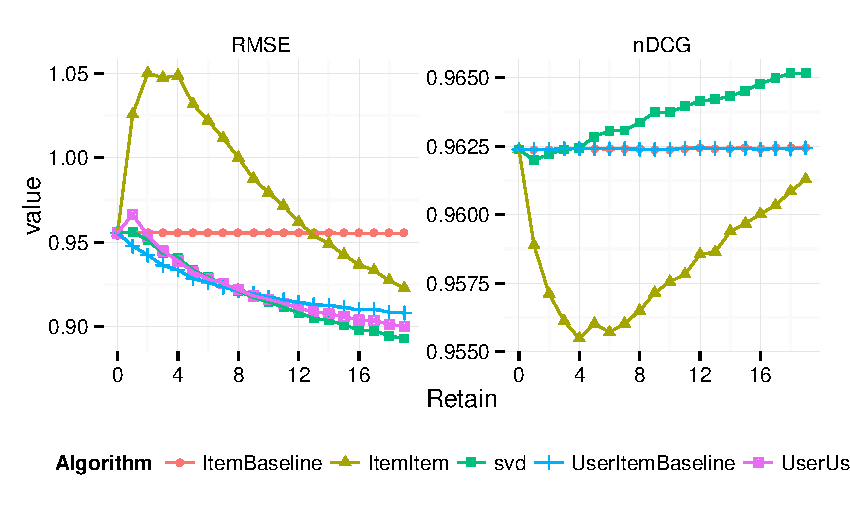
\includegraphics[width=\linewidth]{../lenskit/output/ekstrandTuned20/accuracy.pdf}
  \caption{Left: RMSE, Right: nDCG}
  \label{fig:rmse}
  \label{fig:ndcg}
\end{figure*}
    % RMSE plot
    % point out error bars etc.
    % explain / interpret plot
  Figure \ref{fig:rmse} shows how accurate our algorithms are as measured by RMSE.
  As would be expected the accuracy of our item baseline doesn't change as the amount of information changes.
  The User-User and svd algorithms both perform as expected, starting out with the same accuracy as the item baseline, and then monotonically improving.
  User-User does show a small increase of error with only one rating, but the change is quite small and unlikely to be noticed by users.
  Interestingly, User-User and svd both perform about as well as our smarter user item baseline. %TODO: explain this better

      % explain strangeness of Item-Item
  Item-Item performs quite poorly in the cold start setting.
  Until we have around 20 ratings the RMSE of Item-Item is worse than the item baseline.
  More interestingly, unlike the other algorithms Item-Item actually appears to performs worse as it gets more ratings for the first few ratings.
  
  The curve exhibited by Item-Item's RMSE is caused by two trends.
  First as the system revives more ratings, predictions from Item-Item are more accurate, leading to a downward trend.
  Secondly, as the system revives more ratings, Item-Item can make predictions for more items, meaning the fewer predictions are serviced by the baseline.
  Because the baseline is more accurate, this leads to an upward trend.
  Overall this leads to curved performance.
  If we were to compute RMSE only over the items where item-item can make a prediction we would see a curve similar to the other algorithms, but shifted up.
      % possibly coverage plot
      % true crossing point?

\subsection {Recommendatin quality metrics}
  % Recommendation quality metrics
    % NDCG
  Figure \ref{fig:ndcg} shows the algorithm's performance on the nDCG metric.
  The algorithm's behavior is essentially equivalent to the RMSE behavior.
  Again, User-User has a minor dip on very new users, but then tracks SVD in uniformly improving quite well from there.
  Likewise Item-Item exhibits the same dipped accuracy, although it doesn't catch up the baseline as fast.
  Unlike previous metrics, the item baseline, and the user-item baseline have the same performance.
  This is because nDCG is a ranking metric, not an accuracy metric.
  Because the user item baseline orders items the same way as the item baseline, both will have the same accuracy on any ranking metrics.

    % MAP, precision, fallout plots 
    % explain results from MAP and precision
    % explain recall results
    % recall results, strangeness and popularity


\begin{figure*}[ht!]
  \centering
  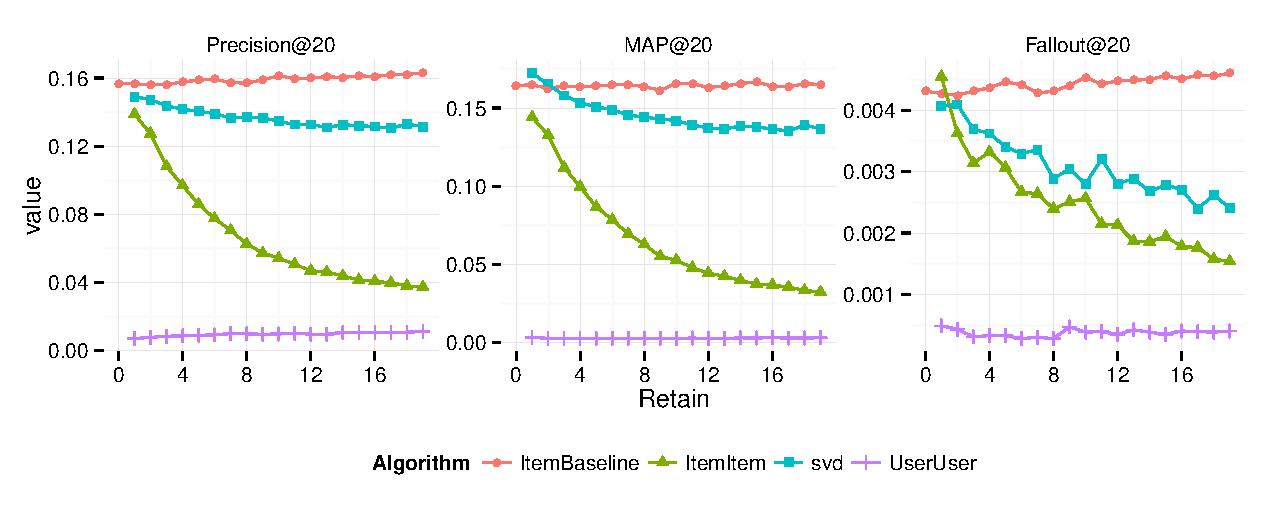
\includegraphics[width=1.1\linewidth]{../lenskit/output/ekstrandTuned20/TopNPrecision.pdf}
  \caption{TODO}
  \label{fig:map}
\end{figure*}


  Figure \ref{fig:map} shows MAP@20, precision@20, and fallout@20.
  All three metrics show essentially the same trend, User-User gets the lowest score, the baselines get the highest score.
  On both MAP@20 and precision@20 svd gets a higher score than Item-Item throughout, performing almost as highly as the baseline.
  On fallout@20 Item-Item performs higher than svd and the baseline, but decreases faster than bath, ending with a lower score than either. 
  We also tried recall@20 and mrr@20 and found the same trend.

  This result is rather strange as MAP and precision are metrics where high scores imply better performance, whereas fallout is a metric where high scores imply poor performance.
  This leads to an issue, these metrics contradict each other in terms of the quality of the recommendations from our algorithm.
  One possible reason for this is that these topN metrics are known to be biased toward recommendations that have more popular items \cite{bellogin}.
  Looking at the average popularity (figure \ref{fig:pop}) of recommended items, we see that the average popularity of the recommendations closely replicates the previous three plots.
  Therefore we seek a different, less biased metric to analyze the quality of the recommendations.


  % TopN average rating / topn rmse
    % interpret graph and reason about what it means about quality

\begin{figure*}[ht!]
  \centering
  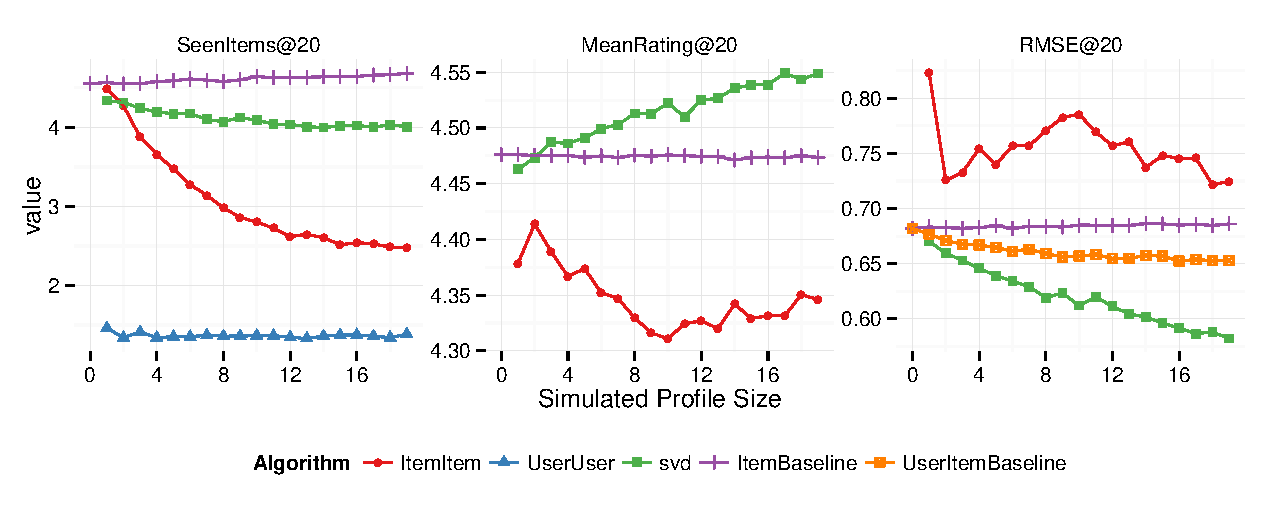
\includegraphics[width=1.1\linewidth]{../lenskit/output/ekstrandTuned20/rmse_20.pdf}
  \caption{TODO}
  \label{fig:topN.rmse}
\end{figure*}

  The first graph in figure \ref{fig:topN.rmse} shows the average number of items in the top 20 recommendations for each algorithm that were also in the test set.
  The average number of test set items in recommendations shows a similar trend to the MAP, precision, and recall metrics, user-user getting by far the fewest seen items, and the baseline getting the most.
  %TODO: talk about trust building here!

  The second graph in figure \ref{fig:topN.rmse} shows the average rating for those items in the top 20 recommendations for each algorithm.
  The first thing to note about this graph is that all of these algorithms are doing a reasonable job of recommending items the user might like to watch, with all algorithms averaging above 4 stars (implying that the recommended items are, at least on average, enjoyable).
  SVD performs as expected, starting at close to the same average rating as the baselines, and then slowing improving as more ratings are entered.
  Item-Item performs poorly, not only performing worse than the baseline, but showing worse performance as more ratings are added.
  This is quite possibly a similar trend to the one we observed with RMSE and nDCG, where Item-Item's performance decreased as coverage increased leading to the curved performance at cold start.
  
  During testing with other values of N for this metric and the next, we found that User-User's behavior compared to the other algorithms changed significantly with different values of N.
  This is probably due to the very low rate of having seen items in the recommendations, which makes its value much less stable, than the other algorithms.
  Because of this behavior we will draw no conclusion from User-User's performance on this metric, to avoid accidentally attributing behavior to it, that was instead formed by our choice of 20 as N.
  
  The third graph in figure \ref{fig:topN.rmse} shows the RMSE our algorithms got on items in the top 20 recommendations for each algorithm.
  Not surprisingly, this figure shows the same trends as the last one meaning that the algorithms whose recommendations were (on average) most likable, were those whose recommendations were most accurate.
  Again, SVD performs quite well, Item-Item shows poor performance, and, due to sensitivity of User-User to our choice of N, we make no conclusions about User-User.

\subsection{Other recommender metrics}
  % Other recommender metrics

\begin{figure*}[ht!]
  \centering
  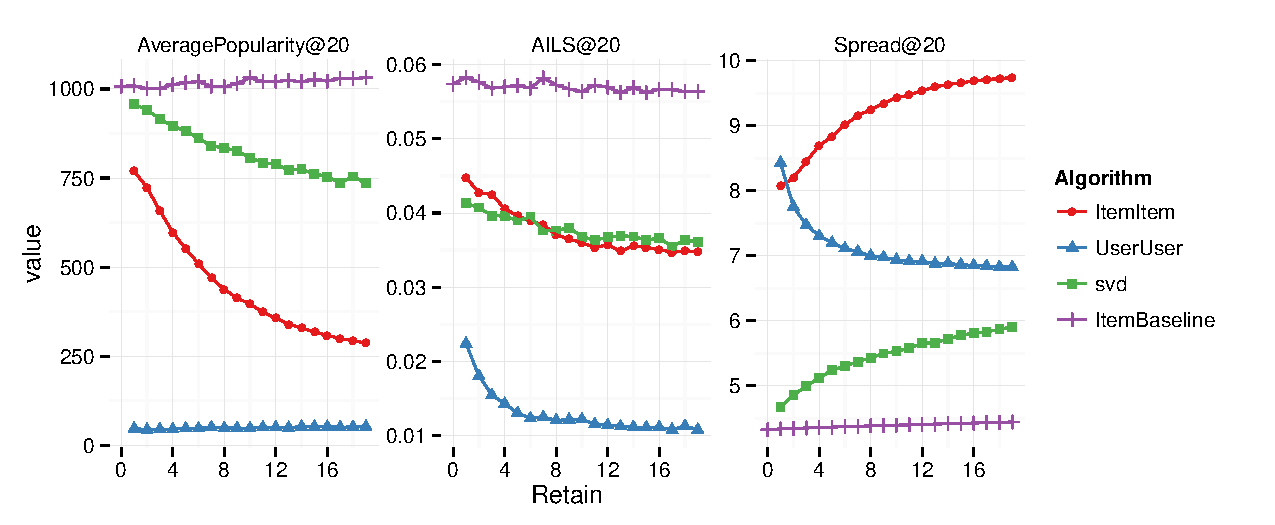
\includegraphics[width=\linewidth]{../lenskit/output/ekstrandTuned20/popdiv.pdf}
  \caption{TODO}
  \label{fig:pop}
\end{figure*}


    % popularity graph
  The first graph in figure \ref{fig:pop} shows the average popularity of recommended items by each algorithm.
  %TODO: re-write this
  Across all datapoint sizes the ranking of algorithms is the same, with the baselines recommending the most popular movies, followed by svd, which recommends less popular movies, then Item-Item, which recommends much less popular movies, leaving User-User to recommend the least popular movies.
  Unfortunately, we don't know of any guideline for understanding how popular users desire their recommendations to be.
  That in mind, we expect that users will feel the baseline's popularity (around 1000) is too high, and User-User's popularity (around 50) is too low.
  SVD and Item-Item both seem to perform well, with SVD generating more popular recommendations, than Item-Item, and both algorithms showing a significant trend to make less popular predictions as we know more about the user.

    % diversity plot
  The diversity graph in \ref{fig:pop} shows a similar trend to the popularity trend with the baseline algorithms producing the least diverse list of recommendations and User-User providing by far the most diverse list of recommendations.
  For the first few ratings SVD is able to provide more diverse recommendations than Item-Item.
  However, Item-Item seems to grow in diversity faster than SVD in response to more data, so after 4 ratings Item-Item is providing slightly more diverse recommendations than SVD.
  Overall, Item-Item and SVD are providing recommendations that, at least in an offline context, appear to have quite comparable diversity.


\begin{figure}[ht!]
  \centering
  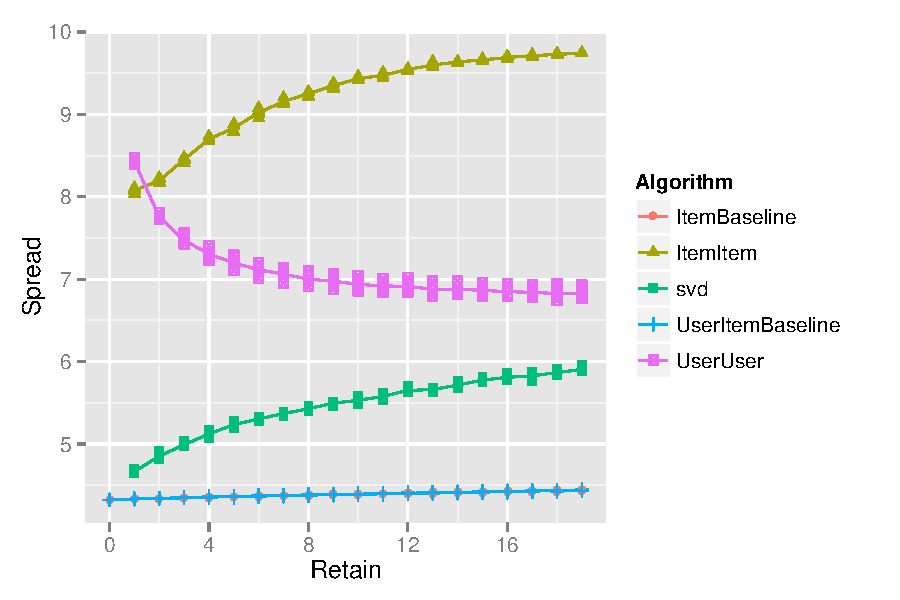
\includegraphics[width=1.1\columnwidth]{../lenskit/output/ekstrandTuned20/topN_entropy.pdf}
  \caption{TODO}
  \label{fig:spread}
\end{figure}


  % spread plot
  The graph in \ref{fig:spread} shows the spread of the recommendations from each algorithm.
  Because this metric can only be computed over a group of people, confidence intervals over the per-user average are not provided, instead the specific spread values computed in each five folds are shown as points, with lines connecting the value from the five metrics.
  %TODO: make this point earier and better.
  Like the diversity and popularity metrics we see that the values take a much larger range, with different algorithms seeming to converge to different amounts spread.
  The baseline algorithms, which recommend every user the same list of recommendations (unless the user has rated one of those items) have the lowest spread.
  SVD has the second lowest spread, starting with a spread very close to the baselines and then slowly growing more spread as it gets more ratings.
  Like popularity, we don't know exactly how much spread is best for a recommender system, but we can guess that we want more spread from our recommendations than baseline, and all other things being equal, more spread is probably better.
  Based on this intuition it seems that SVD might have focus on too few items in its recommendations.

  User-User and Item-Item both have significantly more spread than the other algorithms.
  They show interestingly opposite trends, with User-User providing more spread at one rating, and then decreasing, and Item-Item giving less spread and then increasing.
  By 8 ratings, we see that Item-Item has by far the most spread recommendations.
  It is strange that User-User would get less spread as it learns more about users.
  This implies that the more it learns about users, the less spread out its recommendations are.
  This could be some form of a regression towards the mean, where as it learns more about users its recommendations become less personalized to the users individual quirks.
  More research will be needed to understand this trend.
  
\section{Conclusions}
  % summary of results in a big old table.
    % the accuracy of svd and user-user both seemed good. item-item seemed to have trouble especially with very new users.
    % svd did quite well on our traditional topN metrics, item-item did OK, and user-user did bad., but there are flaws with these metrics.
    % on our topN RMSE item-item (again) seemed to have issues, and user-user did quite well, but the low hit rate is troubleing. 
    % again svd seems the winner here.
    % on our fluffy metrics item-item and svd seemed to do well. I might argue that item-item seemed to do better (spread, and higher throughout).
    % user-user seemed to do poor
  % what this means
    % user-user seems to be able to give accurate predictions, but seems to focus on overly obscure items in recommendation.
    % item-item seems to give not-bad recommendations, but its predictions have issues
    % based only on these results svd seems to be the best performer and is our recommendation to new systems.
  % other takeaways
    % regularization
    % if you use a switching recommender, this methodology can help you choose when to switch.
    % non-traditional metrics can tell you more about what is going on, these seem to be more properties of the class of algo than of the data, so its worth looking at these when choosing algorithms, to find one with properties that are good for your task.

  % limitations and opprotunities
    % dataset limitations
      % only one domain
      % no quitters in our dataset
    % metrics limitations
      % many metrics require user data to help us understand what users want from a recommender
      % no well known ``goodness'' metric for topN.
    % algorithm limitations
      % only covered three common families,
      % different algos tuned specifically for cold start.
      % algos that use extra data about users or about items.

  % despite the limitations we were able to show differences between algorithms in a cold start situation.

\section{Acknowledgements}
 TODO:

\bibliographystyle{abbrv}
\bibliography{resources}  % sigproc.bib is the name of the Bibliography in this case

\end{document}
